\documentclass[tikz,border=7pt]{standalone}
\usepackage{amsmath,amssymb}
\usetikzlibrary{arrows.meta,calc,fit,positioning,backgrounds,decorations.pathreplacing,shapes.geometric}

\begin{document}
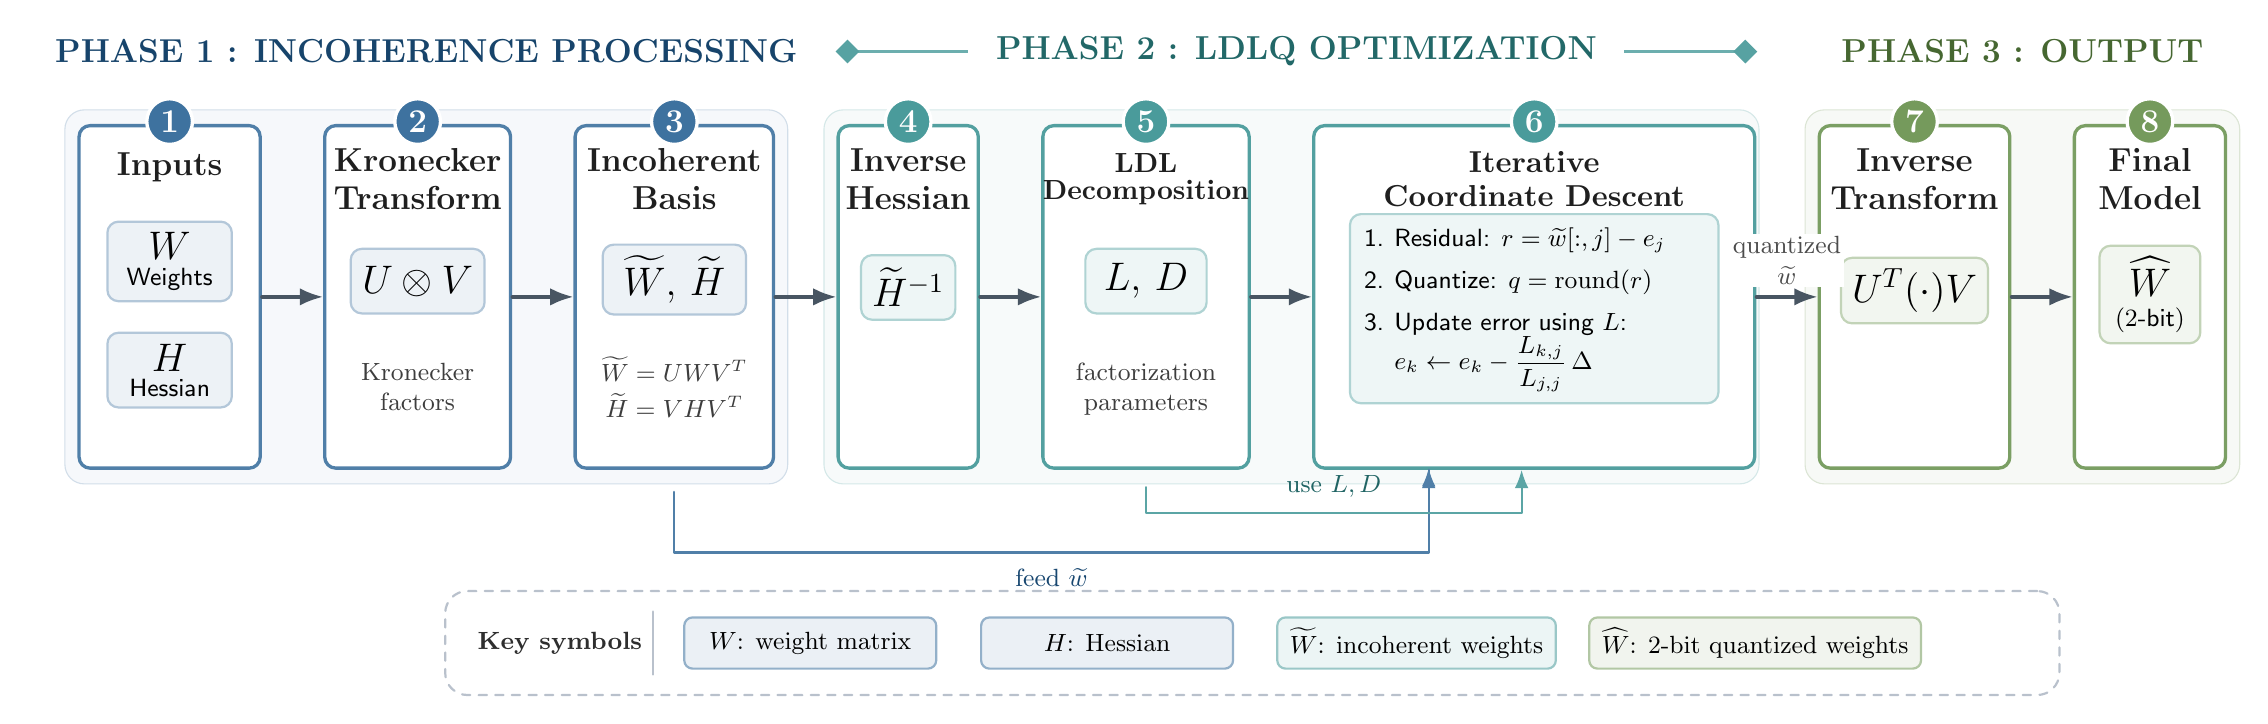
\begin{tikzpicture}[
    x=1cm,y=1cm,
    font=\sffamily,
    >=Latex,
    line cap=round,
    line join=round,
    arrow/.style={-Latex, very thick, draw=ink!82},
    bus/.style={-Latex, thick, draw=ink!70},
    backbus/.style={-Latex, thick, draw=ink!72},
    stage/.style={rounded corners=4pt, very thick, fill=white, minimum height=4.35cm, inner sep=0pt, align=center},
    pone/.style={draw=blueA!78},
    ptwo/.style={draw=tealA!82},
    pthree/.style={draw=greenA!82},
    sub/.style={rounded corners=4pt, thick, align=center, minimum height=0.82cm, inner sep=4pt},
    title/.style={font=\bfseries\large, align=center, text=black!88},
    smalltext/.style={font=\small, align=center, text=black!76},
    tinytext/.style={font=\scriptsize, align=center, text=black!76},
    steplabel/.style={circle, minimum size=0.58cm, inner sep=0pt, fill=#1!86, draw=white, very thick, text=white, font=\bfseries\large},
    phaseLabel/.style={font=\bfseries\large, text=#1!75!black, fill=white, inner xsep=0.35cm},
    legendItem/.style={rounded corners=3pt, draw=#1!48, fill=#1!9, thick, minimum width=3.2cm, minimum height=0.65cm, inner xsep=0.16cm, font=\small, align=center}
]

% Palette.
\definecolor{ink}{HTML}{203040}
\definecolor{blueA}{HTML}{1F5B8F}
\definecolor{tealA}{HTML}{2D8B8B}
\definecolor{greenA}{HTML}{5E8A42}
\definecolor{softBlue}{HTML}{F1F6FC}
\definecolor{softTeal}{HTML}{EFF9F8}
\definecolor{softGreen}{HTML}{F4F8EF}
\definecolor{grayLine}{HTML}{B9C1CC}

% -----------------------
% Explicit layout numbers.
% The x-coordinates are computed from variable node widths plus a fixed gap.
% This keeps the long stage 6 readable without squeezing stages 1--5.
% -----------------------
\def\gap{0.82}
\def\wone{2.30}
\def\wtwo{2.36}
\def\wthree{2.52}
\def\wfour{1.78}
\def\wfive{2.62}
\def\wsix{5.60}
\def\wseven{2.42}
\def\weight{1.92}
\def\stageH{4.35}
\pgfmathsetmacro{\xone}{0}
\pgfmathsetmacro{\xtwo}{\xone + .5*\wone + \gap + .5*\wtwo}
\pgfmathsetmacro{\xthree}{\xtwo + .5*\wtwo + \gap + .5*\wthree}
\pgfmathsetmacro{\xfour}{\xthree + .5*\wthree + \gap + .5*\wfour}
\pgfmathsetmacro{\xfive}{\xfour + .5*\wfour + \gap + .5*\wfive}
\pgfmathsetmacro{\xsix}{\xfive + .5*\wfive + \gap + .5*\wsix}
\pgfmathsetmacro{\xseven}{\xsix + .5*\wsix + \gap + .5*\wseven}
\pgfmathsetmacro{\xeight}{\xseven + .5*\wseven + \gap + .5*\weight}
\def\yc{0}

% Phase backgrounds, behind boxes.
\begin{scope}[on background layer]
  \node[rounded corners=7pt, fill=blueA!4, draw=blueA!20, inner xsep=0.18cm, inner ysep=0.20cm,
        fit={(\xone-1.15,-2.175) (\xthree+1.26,2.175)}] (bg1) {};
  \node[rounded corners=7pt, fill=tealA!4, draw=tealA!20, inner xsep=0.18cm, inner ysep=0.20cm,
        fit={(\xfour-0.89,-2.175) (\xsix+2.675,2.175)}] (bg2) {};
  \node[rounded corners=7pt, fill=greenA!5, draw=greenA!22, inner xsep=0.18cm, inner ysep=0.20cm,
        fit={(\xseven-1.21,-2.175) (\xeight+0.96,2.175)}] (bg3) {};
\end{scope}

% Main stage boxes.
\node[stage,pone,minimum width=\wone cm]   (s1) at (\xone,\yc) {};
\node[stage,pone,minimum width=\wtwo cm]   (s2) at (\xtwo,\yc) {};
\node[stage,pone,minimum width=\wthree cm] (s3) at (\xthree,\yc) {};
\node[stage,ptwo,minimum width=\wfour cm]  (s4) at (\xfour,\yc) {};
\node[stage,ptwo,minimum width=\wfive cm]  (s5) at (\xfive,\yc) {};
\node[stage,ptwo,minimum width=\wsix cm]   (s6) at (\xsix,\yc) {};
\node[stage,pthree,minimum width=\wseven cm] (s7) at (\xseven,\yc) {};
\node[stage,pthree,minimum width=\weight cm] (s8) at (\xeight,\yc) {};

% Number badges.
\foreach \n/\s/\c in {1/s1/blueA,2/s2/blueA,3/s3/blueA,4/s4/tealA,5/s5/tealA,6/s6/tealA,7/s7/greenA,8/s8/greenA}{
  \node[steplabel=\c] at ($ (\s.north) + (0,0.03) $) {\n};
}

% Titles.
\node[title] at ($(s1.north)+(0,-0.55)$) {Inputs};
\node[title] at ($(s2.north)+(0,-0.7)$) {Kronecker\\Transform};
\node[title] at ($(s3.north)+(0,-0.7)$) {Incoherent\\Basis};
\node[title] at ($(s4.north)+(0,-0.7)$) {Inverse\\Hessian};
\node[title, font=\bfseries\fontsize{10}{10}\selectfont]
  at ($(s5.north)+(0,-0.7)$) {LDL\\Decomposition};
\node[title, font=\bfseries\fontsize{11}{12}\selectfont]
  at ($(s6.north)+(0,-0.7)$) {Iterative \\ Coordinate Descent};\node[title] at ($(s7.north)+(0,-0.7)$) {Inverse\\Transform};
\node[title] at ($(s8.north)+(0,-0.7)$) {Final\\Model};

% Stage contents.
\node[sub,draw=blueA!34,fill=blueA!8,minimum width=1.58cm] at ($(s1.center)+(0,0.45)$)
  {\Large $W$\\[-1mm]\small Weights};
\node[sub,draw=blueA!34,fill=blueA!8,minimum width=1.58cm] at ($(s1.center)+(0,-0.93)$)
  {\Large $H$\\[-1mm]\small Hessian};

\node[sub,draw=blueA!34,fill=blueA!8,minimum width=1.70cm] at ($(s2.center)+(0,0.20)$)
  {\Large $U\otimes V$};
\node[smalltext] at ($(s2.center)+(0,-1.14)$) {Kronecker\\factors};

\node[sub,draw=blueA!34,fill=blueA!8,minimum width=1.82cm] at ($(s3.center)+(0,0.22)$)
  {\Large $\widetilde W,\,\widetilde H$};
\node[smalltext] at ($(s3.center)+(0,-1.15)$)
  {$\widetilde W=U W V^{T}$\\[0.7mm]$\widetilde H=V H V^{T}$};

\node[sub,draw=tealA!38,fill=tealA!8,minimum width=1.08cm] at ($(s4.center)+(0,0.12)$)
  {\Large $\widetilde H^{-1}$};

\node[sub,draw=tealA!38,fill=tealA!8,minimum width=1.54cm] at ($(s5.center)+(0,0.20)$)
  {\Large $L,\,D$};
\node[smalltext] at ($(s5.center)+(0,-1.17)$) {factorization\\parameters};

\node[sub,draw=tealA!38,fill=tealA!8,minimum width=4.68cm,minimum height=2.02cm,align=left] (icdcore)
  at ($(s6.center)+(0,-0.15)$)
  {\begin{minipage}{4.32cm}\small
    \begin{tabular}{@{}r@{\hspace{0.40em}}p{3.66cm}@{}}
      1. & Residual: $r=\widetilde w[:,j]-e_j$ \\[1.5mm]
      2. & Quantize: $q=\operatorname{round}(r)$ \\[1.5mm]
      3. & Update error using $L$:\\[-0.5mm]
         & $e_k\leftarrow e_k-\dfrac{L_{k,j}}{L_{j,j}}\,\Delta$
    \end{tabular}
  \end{minipage}};

\node[sub,draw=greenA!38,fill=greenA!8,minimum width=1.55cm] at ($(s7.center)+(0,0.08)$)
  {\Large $U^{T}(\cdot)V$};

\node[sub,draw=greenA!38,fill=greenA!8,minimum width=1.28cm] at ($(s8.center)+(0,0.03)$)
  {\Large $\widehat W$\\[-0.5mm]\small $(2\text{-bit})$};

% Main flow arrows.
\draw[arrow] (s1.east) -- (s2.west);
\draw[arrow] (s2.east) -- (s3.west);
\draw[arrow] (s3.east) -- (s4.west);
\draw[arrow] (s4.east) -- (s5.west);
\draw[arrow] (s5.east) -- (s6.west);
\draw[arrow] (s6.east) -- node[above=3pt,font=\small,text=black!70,align=center,fill=white,inner sep=1pt] {quantized\\$\widetilde w$} (s7.west);
\draw[arrow] (s7.east) -- (s8.west);

% Lower bypass buses into coordinate descent.
\coordinate (busWstart) at ($(s3.south)+(0,-0.28)$);
\coordinate (busWmid)   at ($(s3.south)+(0,-1.05)$);
\coordinate (busWend)   at ($(s6.south)+(-1.34,-1.05)$);
\coordinate (busWin)    at ($(s6.south)+(-1.34,0.00)$);
\draw[backbus,draw=blueA!78] (busWstart) -- (busWmid) -- node[below=2pt,font=\small,text=blueA!78!black] {feed $\widetilde w$} (busWend) -- (busWin);
\draw[backbus,draw=blueA!78] (busWin) -- ($(s6.south)+(-1.34,0.02)$);

\coordinate (busLDstart) at ($(s5.south)+(0,-0.22)$);
\coordinate (busLDmid)   at ($(s5.south)+(0,-0.55)$);
\coordinate (busLDend)   at ($(s6.south)+(-0.16,-0.55)$);
\coordinate (busLDin)    at ($(s6.south)+(-0.16,0.00)$);
\draw[backbus,draw=tealA!78] (busLDstart) -- (busLDmid) -- node[above=2pt,font=\small,text=tealA!72!black] {use $L,D$} (busLDend) -- (busLDin);

% Phase bars.
\def\barY{3.10}
\draw[very thick,blueA!70] ($(s1.north west)+(0.14,0.92)$) -- ($(s3.north east)+(-0.14,0.92)$);
\node[diamond,fill=blueA!80,inner sep=2.2pt] at ($(s1.north west)+(0.14,0.92)$) {};
\node[diamond,fill=blueA!80,inner sep=2.2pt] at ($(s3.north east)+(-0.14,0.92)$) {};
\node[phaseLabel=blueA] at ($($(s1.north west)+(0.14,0.92)$)!0.5!($(s3.north east)+(-0.14,0.92)$)$) {PHASE 1 : INCOHERENCE PROCESSING};

\draw[very thick,tealA!70] ($(s4.north west)+(0.14,0.92)$) -- ($(s6.north east)+(-0.14,0.92)$);
\node[diamond,fill=tealA!80,inner sep=2.2pt] at ($(s4.north west)+(0.14,0.92)$) {};
\node[diamond,fill=tealA!80,inner sep=2.2pt] at ($(s6.north east)+(-0.14,0.92)$) {};
\node[phaseLabel=tealA] at ($($(s4.north west)+(0.14,0.92)$)!0.5!($(s6.north east)+(-0.14,0.92)$)$) {PHASE 2 : LDLQ OPTIMIZATION};

\draw[very thick,greenA!70] ($(s7.north west)+(0.14,0.92)$) -- ($(s8.north east)+(-0.14,0.92)$);
\node[diamond,fill=greenA!80,inner sep=2.2pt] at ($(s7.north west)+(0.14,0.92)$) {};
\node[diamond,fill=greenA!80,inner sep=2.2pt] at ($(s8.north east)+(-0.14,0.92)$) {};
\node[phaseLabel=greenA] at ($($(s7.north west)+(0.14,0.92)$)!0.5!($(s8.north east)+(-0.14,0.92)$)$) {PHASE 3 : OUTPUT};

% Legend.
\node[rounded corners=8pt, draw=grayLine, dashed, thick, minimum width=20.5cm, minimum height=1.32cm, inner sep=0pt]
  (legendbox) at ($(s5.south)+(1.35,-2.20)$) {};
\node[font=\bfseries\small, text=black!82, anchor=west] at ($(legendbox.west)+(0.3,0)$) {Key symbols};
\draw[grayLine, thick] ($(legendbox.west)+(2.65,-0.40)$) -- ($(legendbox.west)+(2.65,0.40)$);
\node[legendItem=blueA]  at ($(legendbox.west)+(4.65,0)$) {$W$: weight matrix};
\node[legendItem=blueA]  at ($(legendbox.west)+(8.42,0)$) {$H$: Hessian};
\node[legendItem=tealA]  at ($(legendbox.west)+(12.35,0)$) {$\widetilde W$: incoherent weights};
\node[legendItem=greenA] at ($(legendbox.west)+(16.65,0)$) {$\widehat W$: 2-bit quantized weights};

\end{tikzpicture}
\end{document}
